%-----------------------------------------------------------------------------
%	PACKAGES AND DOCUMENT CONFIGURATIONS
%-----------------------------------------------------------------------------

\documentclass{article}

\usepackage{graphicx} % Required for the inclusion of images
\usepackage{natbib} % Required to change bibliography style to APA
\usepackage{amsmath} % Required for some math elements
\usepackage{amssymb}
\usepackage{grffile}
\usepackage[export]{adjustbox}
\usepackage{subcaption}
\usepackage{float}
\usepackage{listings}
\usepackage[margin=1.0in]{geometry}
\usepackage{tikz}
\usepackage{enumitem}
\usepackage{scrextend}
\usepackage{siunitx}
\usepackage{minted}

\usetikzlibrary{shapes.geometric, arrows}
\tikzstyle{startstop} = [rectangle, rounded corners, minimum width=1cm, minimum height=1cm,text centered, draw=black, fill=white!30]
\tikzstyle{process} = [rectangle, minimum width=1.5cm, minimum height=1cm, text centered, draw=black, fill=white!30]
\tikzstyle{arrow} = [thick,<->,>=stealth]

\renewcommand{\baselinestretch}{1.5}
\setlength\parindent{0pt} % Removes all indentation from paragraphs

%-----------------------------------------------------------------------------
%	DOCUMENT INFORMATION
%-----------------------------------------------------------------------------

\title{ECE 547 Project 1} % Title

\author{Yang \textsc{Wang}}  % Author name

\date{\today} % Date for the report

\renewcommand{\theenumi}{\alph{enumi}} % use letters for list items

\begin{document}

\maketitle % Insert the title, author and date

%-----------------------------------------------------------------------------
%	Problems
%-----------------------------------------------------------------------------

\section*{Part 1}
	\begin{enumerate}
		\item The MATLAB code for simulating M/M/1 queue is listed in Appendix.
		\item Plot $P_n$ against $n$ when $\lambda = 5$ and $\mu = 6$. As one could
			observe, the simulation result matches closely with the theoretical result
			from using Little's Law as shown in Figure 1.
			\begin{figure}[!hbt]
				\centering
				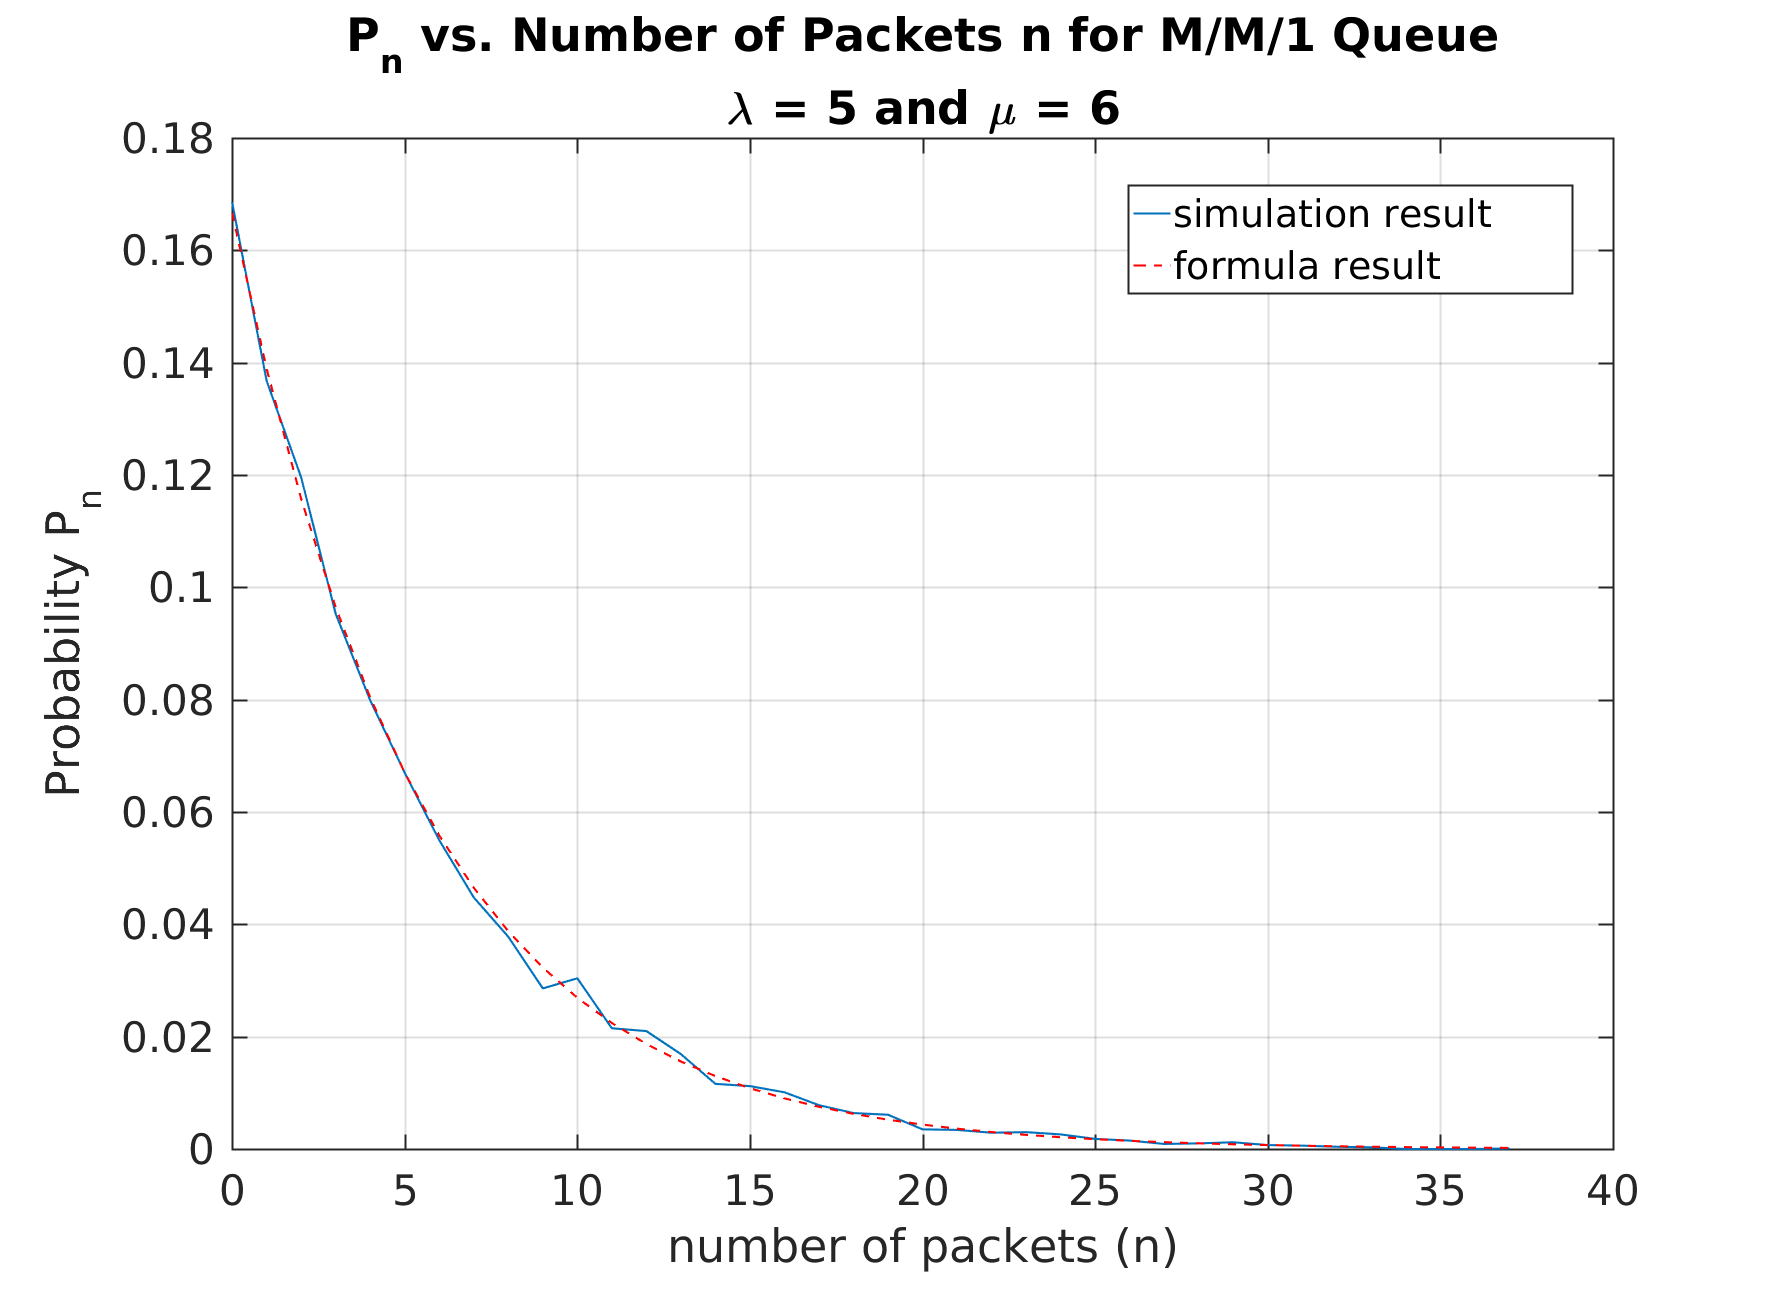
\includegraphics[width=0.8\linewidth]{proj1_p1_pn_vs_n.png}
				\caption{$P_n$ against $n$ when $\lambda = 5$ and $\mu = 6$.}
			\end{figure}
		\item $E[n] = 4.960012$ for the simulated M/M/1 queueing system.
		\item $E[T] = 1.004138$ for the simulated M/M/1 queueing system.
	\end{enumerate}

\section*{Part 2}
	\begin{enumerate}
		\item The MATLAB code for generating an Erlang random variables is listed in
			Appendix. The estimation of $P(X > x)$ is plotted in Figure 2.
			\begin{figure}[!hbt]
				\centering
				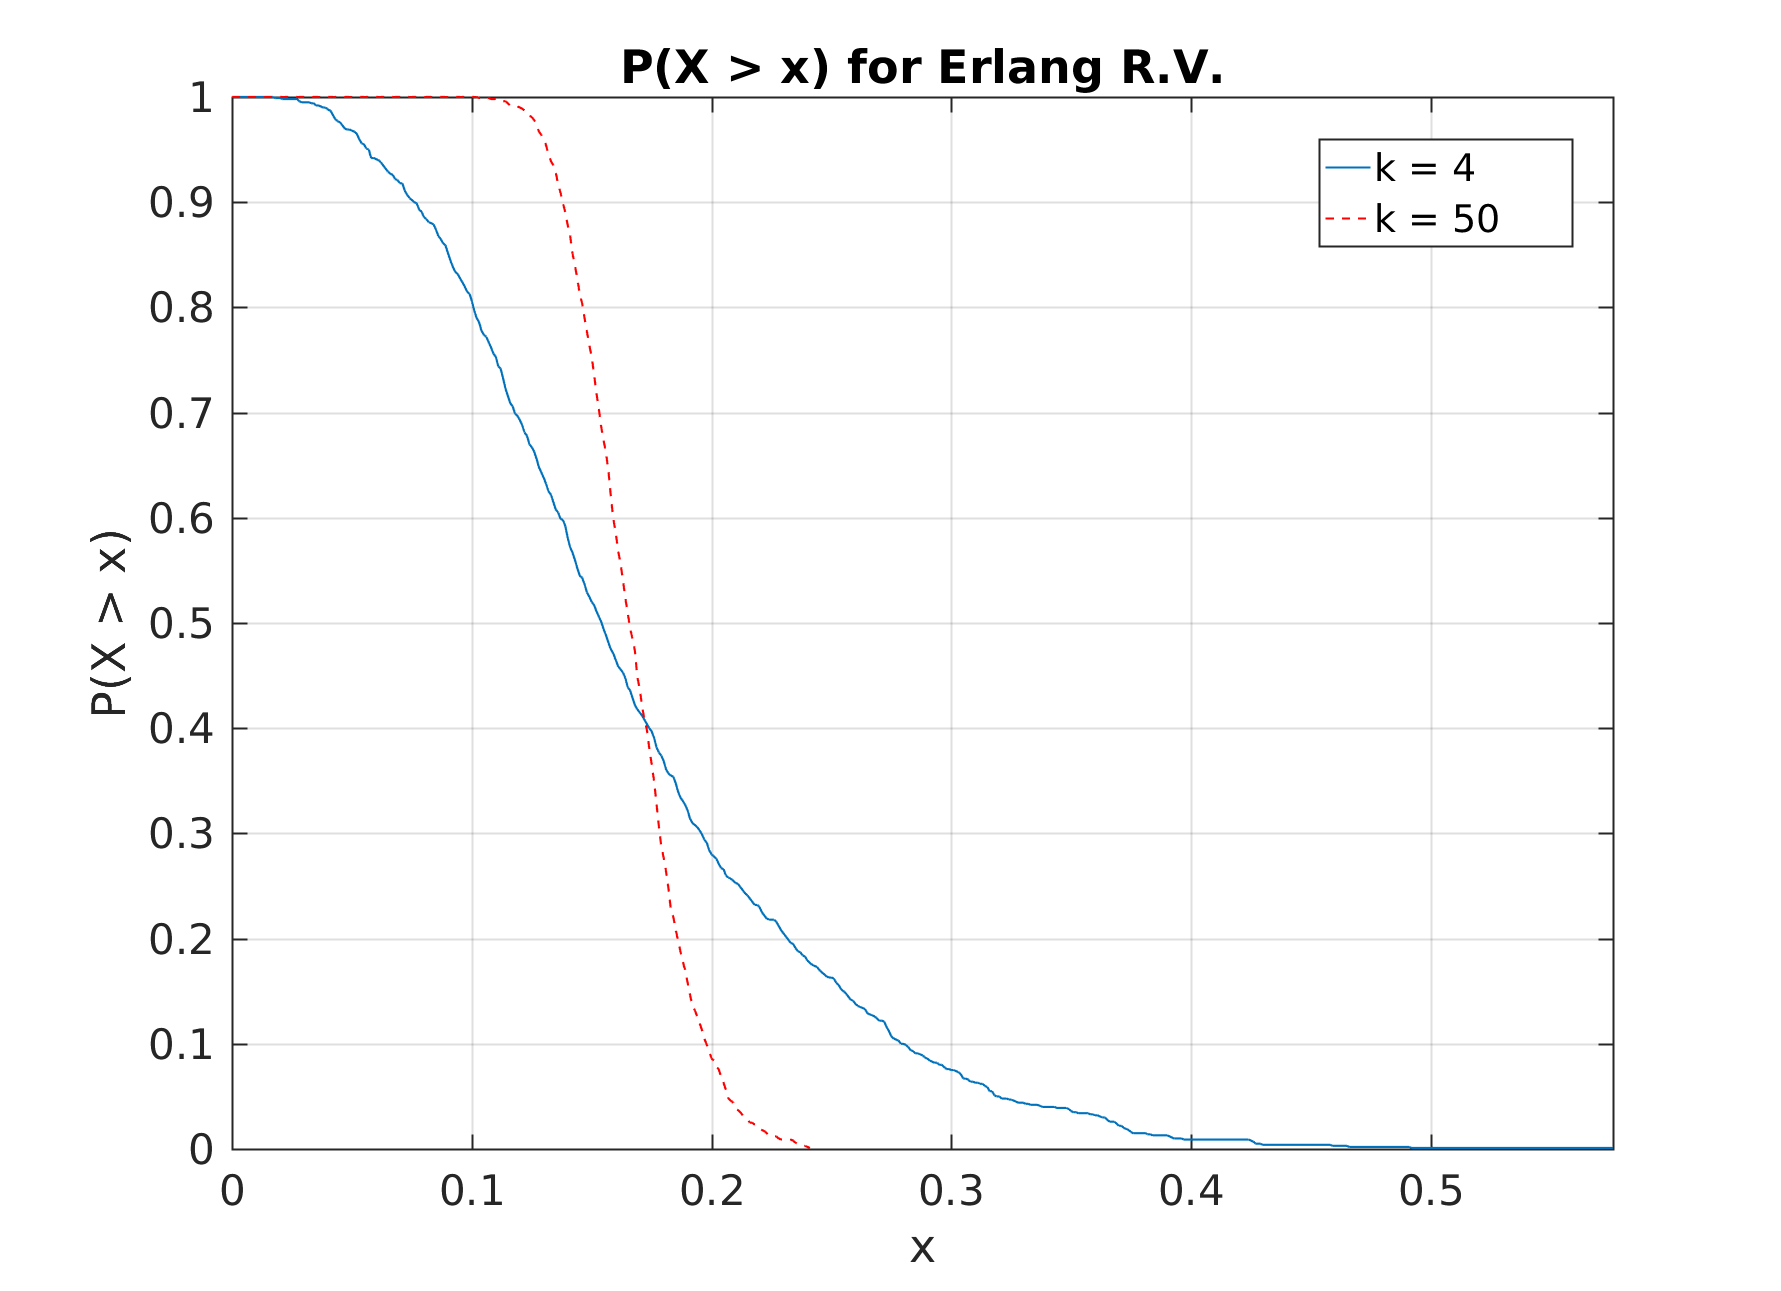
\includegraphics[width=0.8\linewidth]{proj1_p2_px.png}
				\caption{$P(X > x)$ for Erlang random variables for different values of $k$.}
			\end{figure}
		\item The MATLAB code for M/$E_k$/1 simulation is identical as the code used
			for M/M/1 queue simulation except that now the service time is an Erlang
			random variable. Please see Appendix for the detailed code listing.
		\item $E[n] = 3.372888$. The expected number of packets in the queueing
			system with Erlang service rate is \textbf{less than} the queueing system
			with Exponential service rate. The simulated expected delay $E[T] = 0.671119$
			is also smaller. As one could expect this result, since as $k$ increases,
			the M/$E_k$/1 queue is converging into more of a M/D/1 queue. Figure 3
			shows the probability $P_n$ against $n$.
			\begin{figure}[!hbt]
				\centering
				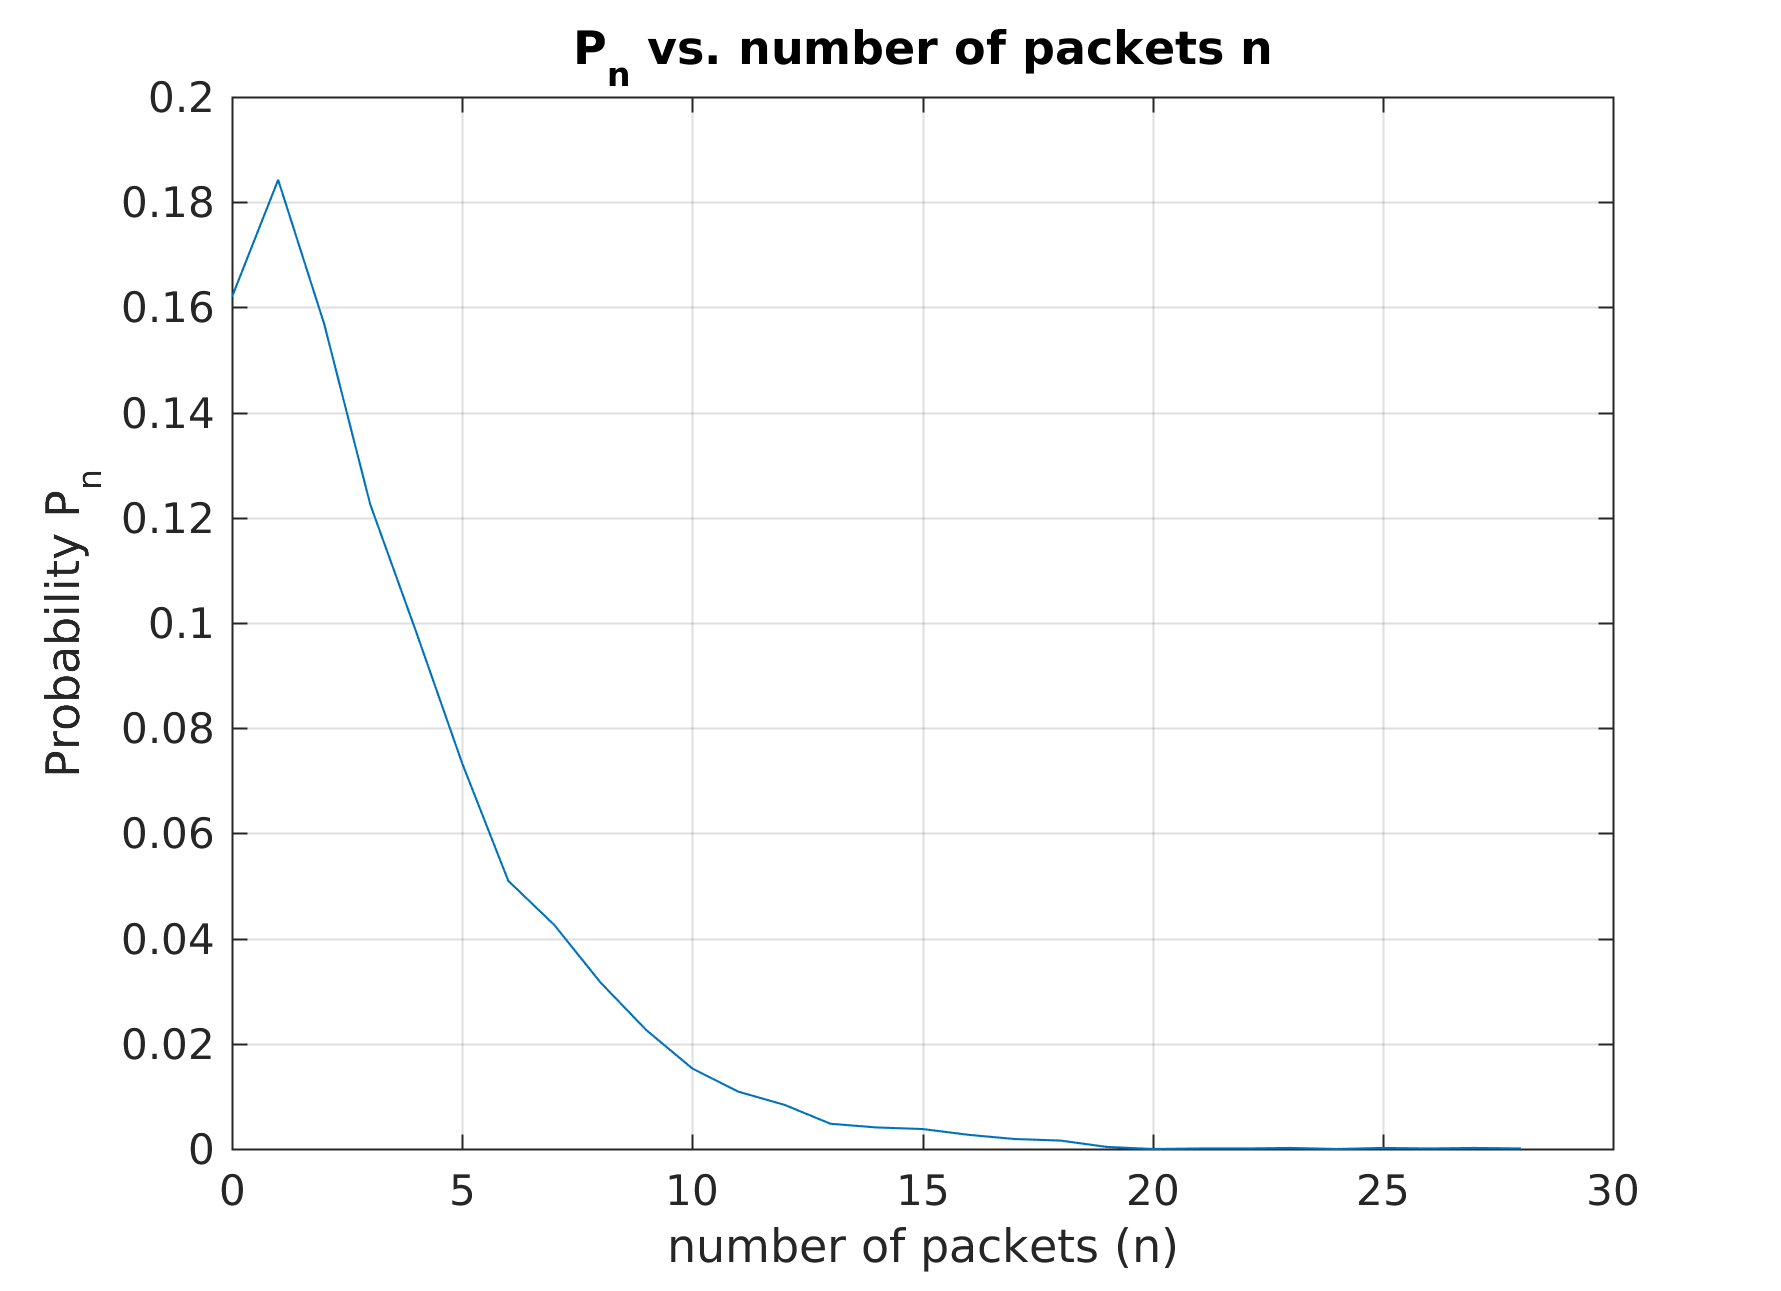
\includegraphics[width=0.8\linewidth]{proj1_p2_pn_vs_n.png}
				\caption{$P_n$ against $n$ for M/$E_k$/1 with $\lambda = 5$ and $k = 4$.}
			\end{figure}
		\item For the simulation, the following parameters are chosen:
			\begin{align*}
				k &= 50 \\
				D &= \frac{1}{6}
			\end{align*}
			And $\lambda$ is a MATLAB row vector that goes from 1 to 6 with interval
			0.6. Hence, a total number of 10 expected number of packets versus each
			utilization value $\rho$ for the two queueing system is calculated.
			Please refer to Appendix for the detailed simulation code. Figure 4 shows
			the the utilization versus the expected number of packets for M/D/1 queue
			and M/$E_k$/1 queue.
			\begin{figure}[!hbt]
				\centering
				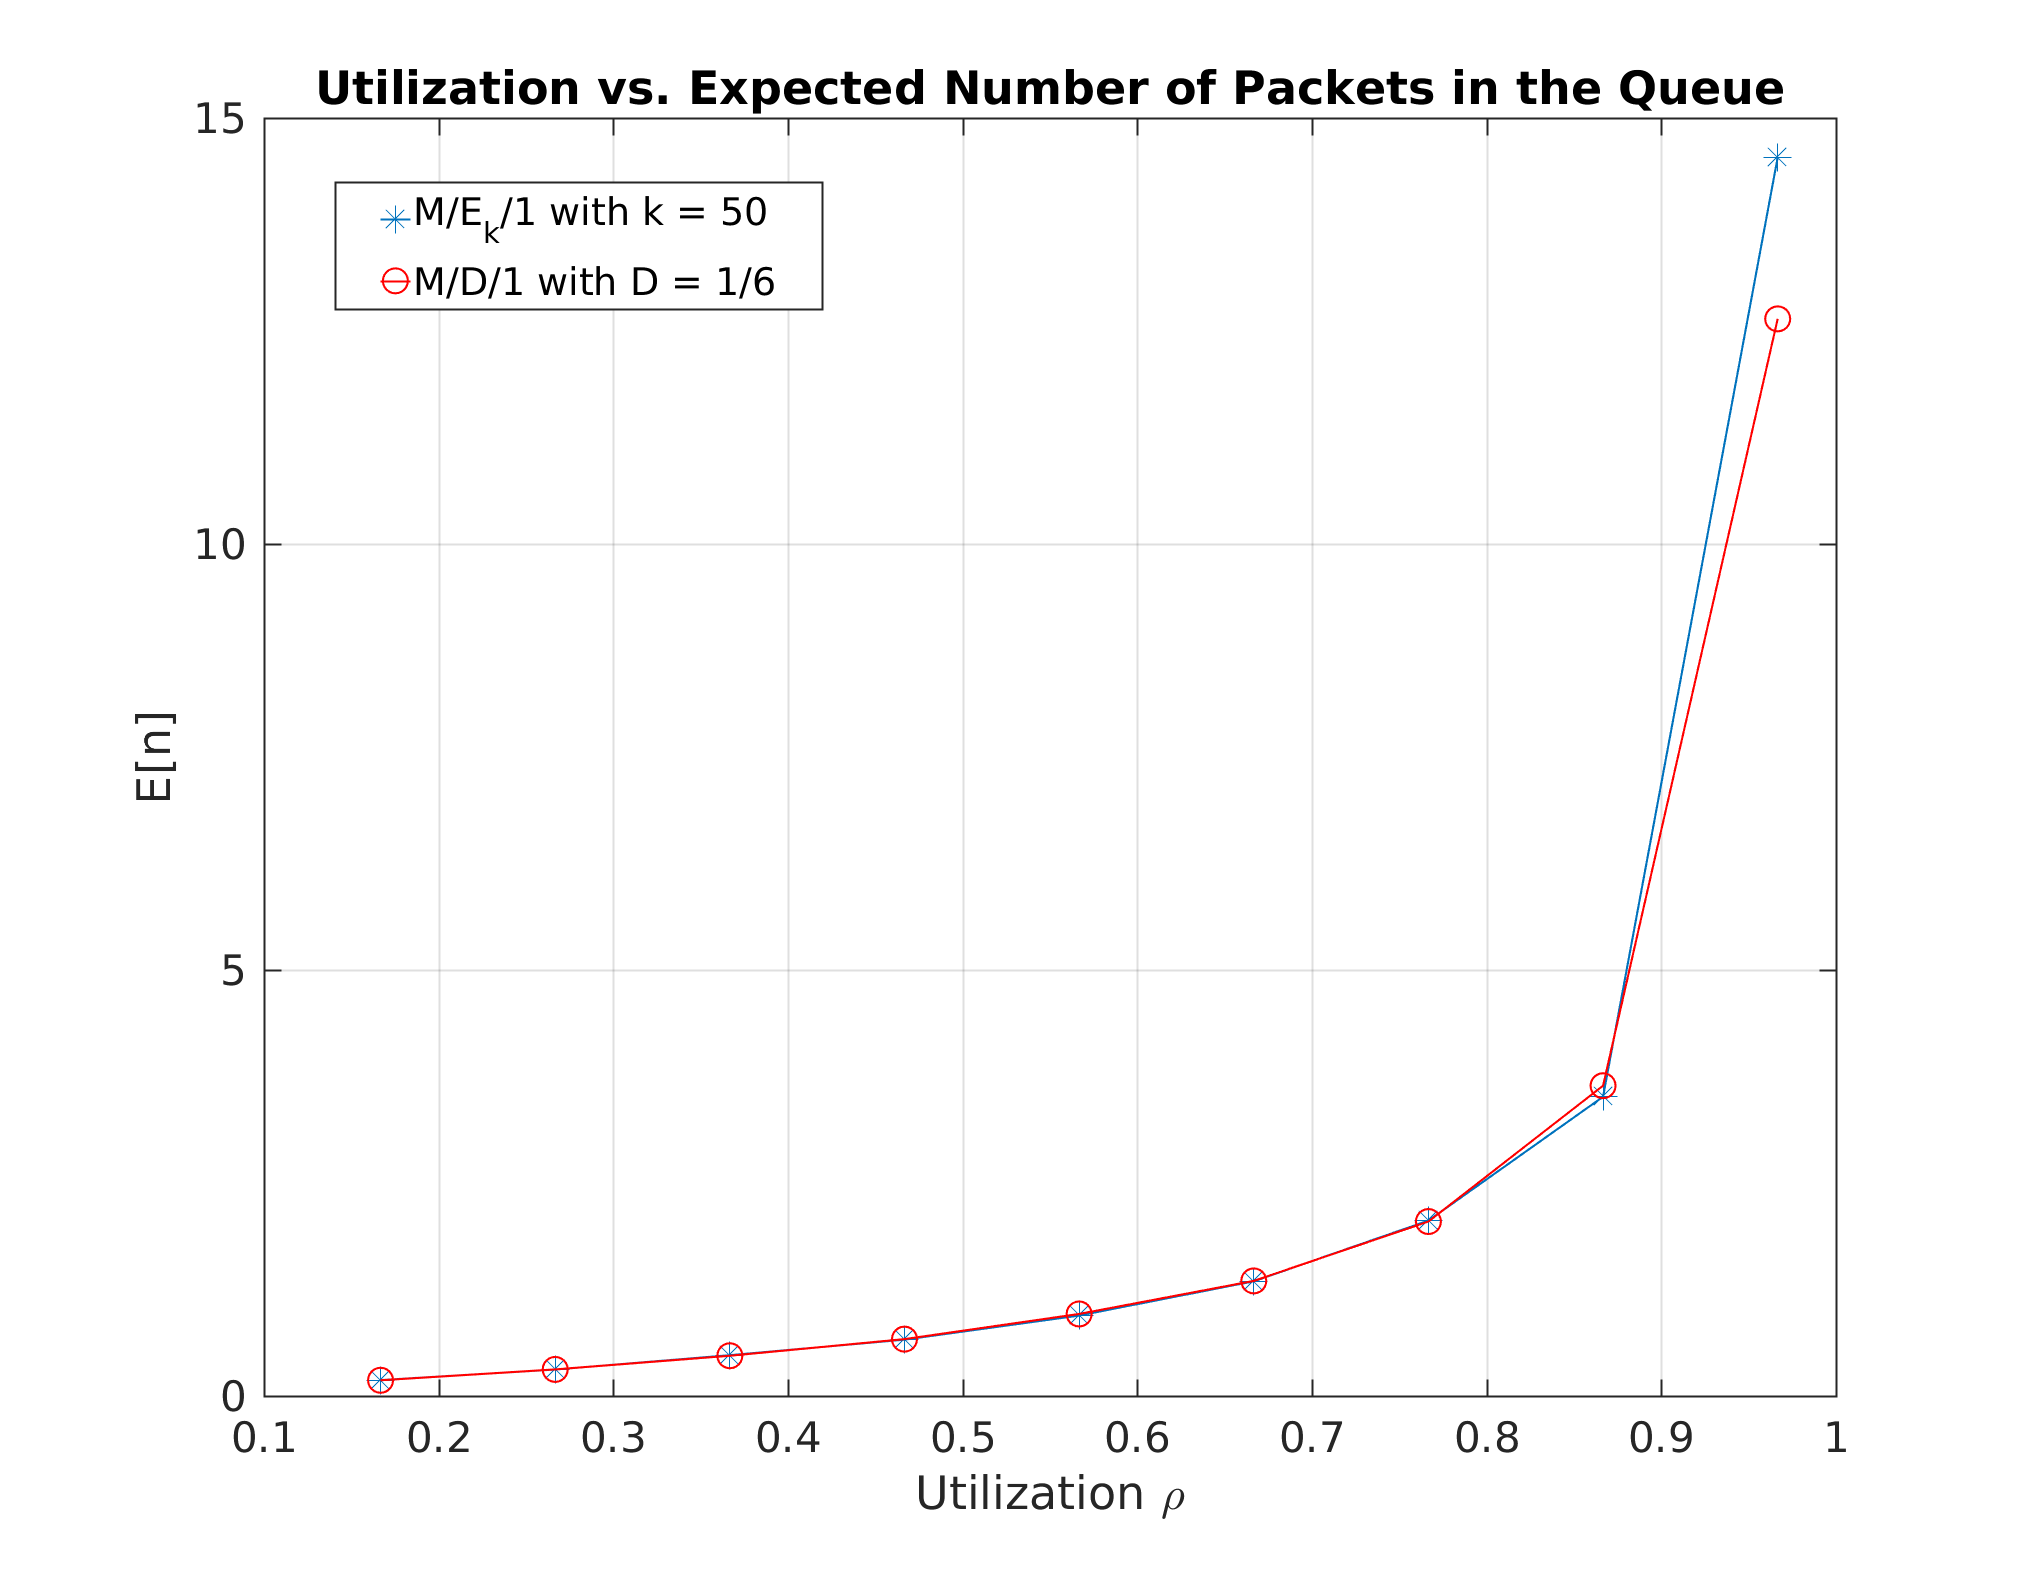
\includegraphics[width=0.7\linewidth]{proj1_p2_en.png}
				\caption{Utilization $\rho$ versus the expected number of packets $E[n]$.}
			\end{figure}
	\end{enumerate}

\section*{Appendix}
	\subsection*{Code Listing}
		\subsubsection*{proj1\_p1.m}
			\inputminted[tabsize=2,breaklines]{matlab}{proj1_p1.m}
		\pagebreak
		\subsubsection*{proj2\_p1.m}
			\inputminted[tabsize=2,breaklines]{matlab}{proj1_p2.m}
		\pagebreak
		\subsubsection*{customer.m}
			\inputminted[tabsize=2,breaklines]{matlab}{customer.m}
		\pagebreak
		\subsubsection*{erlang\_rv.m}
			\inputminted[tabsize=2,breaklines]{matlab}{erlang_rv.m}
\end{document}
